\documentclass[aspectratio=1610,10pt]{beamer}

% \usetheme[progressbar=frametitle]{metropolis}
\usepackage{appendixnumberbeamer}
\usepackage{booktabs}
\usepackage{xspace}
\usepackage{babel}
\usepackage[utf8]{inputenc}
\usepackage{lmodern}
\usepackage{graphicx,caption,subcaption}

\title[]{Distributed Novelty Detection at the Edge for IoT Network Security}
\author{Luís Puhl \and Guilherme Weigert Cassales \and Helio Crestana Guardia \and Hermes Senger}
\institute{Universidade Federal de São Carlos, Brasil\\\url{https://www2.ufscar.br/}}
\date{\today}

\begin{document}

\maketitle

\begin{frame}[noframenumbering]{Contents}
  \setbeamertemplate{section in toc}[sections numbered]
  \tableofcontents[hideallsubsections]
\end{frame}

\section{Introdução}
\begin{frame}{Introdução - Cenário}
  \begin{figure}\centering
    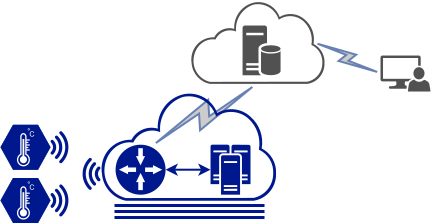
\includegraphics[width=0.7\linewidth]{figures/mfog-arch-fisica.png}
    \caption{Visão geral de IoT, Névoa e Nuvem.}
    \fonte{O autor.}
  \end{figure}
\end{frame}

\section{Estado da Arte e Trabalhos Relacionados}
\begin{frame}[fragile]{Estado da Arte e Trabalhos Relacionados}
\begin{alertblock}{Sistemas de detecção de intrusão em redes}
  \begin{itemize}%[<+- | alert@+>]
    \item Ferramenta BigFlow \cite{Viegas2019}:
    \begin{itemize}
      \item Sistema de detecção de intrusão por anomalia para redes de alta velocidade;
      \item[$\boldsymbol{+}$] Integração da extração dos descritores de fluxo à emissão de alarmes;
      \item[$\boldsymbol{+}$] Capacidade de tratamento de grandes volumes;
      \item[$\boldsymbol{-}$] Atualização semanal com avaliação de um especialista;
      \item[$\boldsymbol{-}$] Execução somente em nuvem.
    \end{itemize}
  \end{itemize}
\end{alertblock}

Network Intrusion Detection based on Machine Learning is not a novel concept.
The plethora of network applications and ways of exploiting them motivate using automated means to detect known and novel attacks. 
% the interest of teach a machine how to detect a novel attack is formed.
There are, though, open questions and challenges on this subject, such as
reducing the false positive rate and detecting attacks in a timely fashion \cite{DaCosta2019a}.

\end{frame}

\begin{frame}[fragile]{Resultados - Variação Processadores}
  \begin{figure}
    \centering
    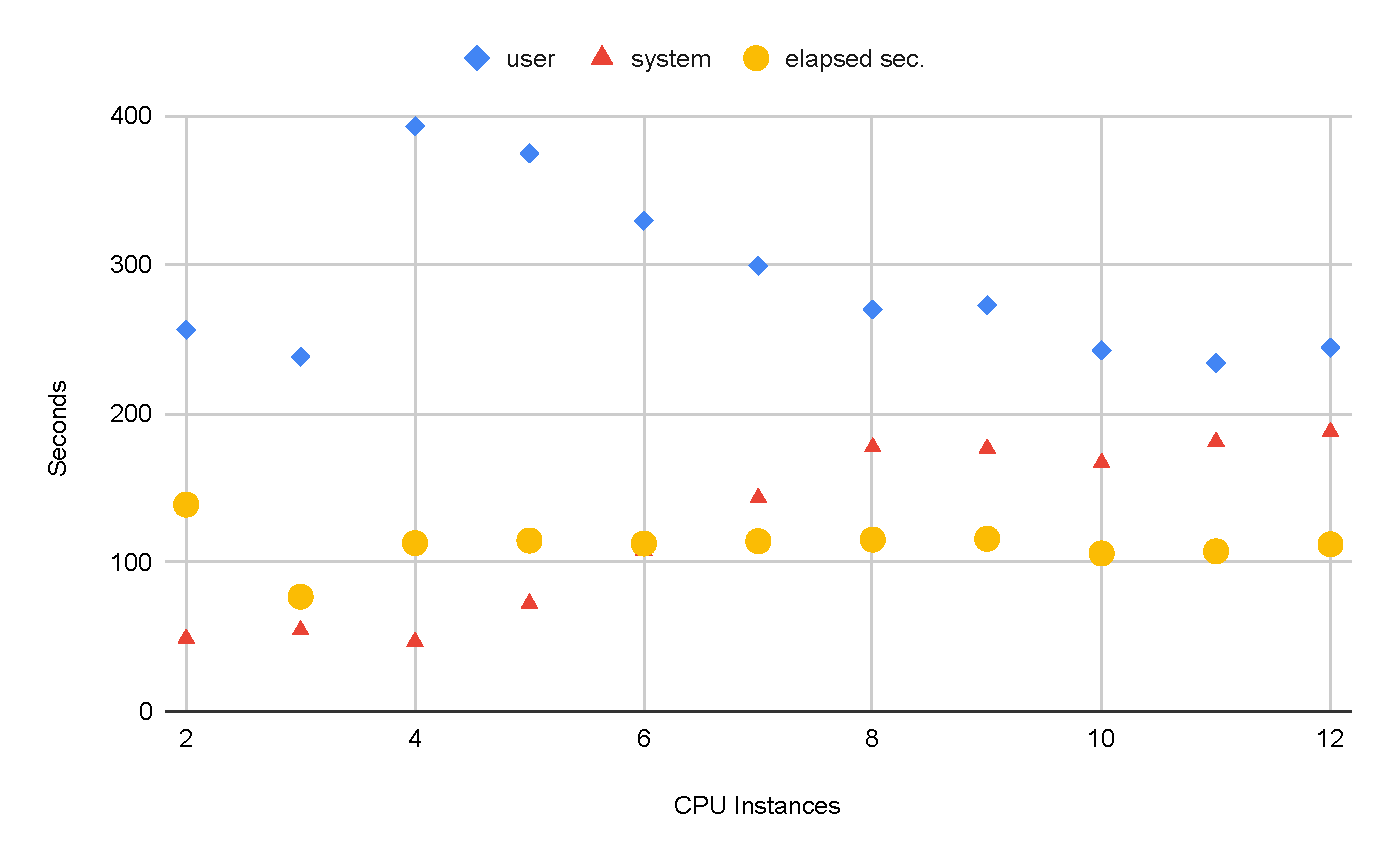
\includegraphics[width=0.7\linewidth,page=1]{experiments/speedup-clean.pdf}
    \caption{Métricas de tempo para execuções do mfog com variação no número de processadores.}
    \label{fig:speedup}
    \fonte{O autor.}
  \end{figure}
\end{frame}

\section{Conclusão}
\begin{frame}{Conclusão}
  
  \begin{alertblock}{Resultados obtidos:}
  \begin{itemize}%[<+- | alert@+>]
    \item Algoritmo minas distribuído e a arquitetura arch
    implementada com modificações;
    \item Distribuição tem pequeno efeito sobre as métricas de qualidade;
    \begin{itemize}
      \item Maior efeito é a redução de etiquetas novidade na versão distribuída;
    \end{itemize}
    \item Resultados mostram que a implementação mfog não atinge escala pelo CCR e eficiência;
  \end{itemize}
  \end{alertblock}
\end{frame}

\begin{frame}[allowframebreaks]{Bibliography}
  \bibliographystyle{splncs04.bst}
  \bibliography{99-refs-ISCC}
\end{frame}

\appendix
{\setbeamercolor{palette primary}{fg=black, bg=yellow}\begin{frame}[standout]
  Appendix
\end{frame}}
\begin{frame}\centering
  \includegraphics[width=0.8\linewidth]{figures/arq-mfog.png}
\end{frame}

\end{document}
